\documentclass[annotation,specification]{itmo-student-thesis}

%% Опции пакета:
%% - specification - если есть, генерируется задание, иначе не генерируется
%% - annotation - если есть, генерируется аннотация, иначе не генерируется
%% - times - делает все шрифтом Times New Roman, требует пакета pscyr.

%% Делает запятую в формулах более интеллектуальной, например: 
%% $1,5x$ будет читаться как полтора икса, а не один запятая пять иксов. 
%% Однако если написать $1, 5x$, то все будет как прежде.
\usepackage{icomma}

\usepackage{color}
\definecolor{lightgray}{rgb}{.9,.9,.9}
\definecolor{darkgray}{rgb}{.4,.4,.4}
\definecolor{purple}{rgb}{0.65, 0.12, 0.82}
\definecolor{dkgreen}{rgb}{0,0.6,0}
\definecolor{gray}{rgb}{0.5,0.5,0.5}
\definecolor{mauve}{rgb}{0.58,0,0.82}
\graphicspath{ {images/} }

\newcolumntype{L}{>{\arraybackslash}m{2.2cm}}
\newcolumntype{K}{>{\arraybackslash}m{4.8cm}} 

%% Поддержка R
\lstset{ %
  language=R,                     % the language of the code
  basicstyle=\footnotesize,       % the size of the fonts that are used for the code
  numbers=left,                   % where to put the line-numbers
  numberstyle=\tiny\color{gray},  % the style that is used for the line-numbers
  stepnumber=1,                   % the step between two line-numbers. If it's 1, each line
                                  % will be numbered
  numbersep=5pt,                  % how far the line-numbers are from the code
  backgroundcolor=\color{white},  % choose the background color. You must add \usepackage{color}
  showspaces=false,               % show spaces adding particular underscores
  showstringspaces=false,         % underline spaces within strings
  showtabs=false,                 % show tabs within strings adding particular underscores
  frame=single,                   % adds a frame around the code
  rulecolor=\color{black},        % if not set, the frame-color may be changed on line-breaks within not-black text (e.g. commens (green here))
  tabsize=2,                      % sets default tabsize to 2 spaces
  captionpos=b,                   % sets the caption-position to bottom
  breaklines=true,                % sets automatic line breaking
  breakatwhitespace=false,        % sets if automatic breaks should only happen at whitespace
  title=\lstname,                 % show the filename of files included with \lstinputlisting;
                                  % also try caption instead of title
  keywordstyle=\color{blue},      % keyword style
  commentstyle=\color{dkgreen},   % comment style
  stringstyle=\color{mauve},      % string literal style
  escapeinside={\%*}{*)},         % if you want to add a comment within your code
  morekeywords={*,...}            % if you want to add more keywords to the set
} 


%% Поддержка JavaScript
\lstdefinelanguage{JavaScript}{
  keywords={typeof, new, true, false, catch, function, return, null, catch, switch, var, if, in, while, do, else, case, break},
  keywordstyle=\color{blue}\bfseries,
  ndkeywords={class, export, boolean, throw, implements, import, this},
  ndkeywordstyle=\color{darkgray}\bfseries,
  identifierstyle=\color{black},
  sensitive=false,
  comment=[l]{//},
  morecomment=[s]{/*}{*/},
  commentstyle=\color{purple}\ttfamily,
  stringstyle=\color{red}\ttfamily,
  morestring=[b]',
  morestring=[b]"
}

\lstset{
   language=JavaScript,
   backgroundcolor=\color{lightgray},
   extendedchars=true,
   basicstyle=\footnotesize\ttfamily,
   showstringspaces=false,
   showspaces=false,
   numbers=left,
   numberstyle=\footnotesize,
   numbersep=9pt,
   tabsize=2,
   breaklines=true,
   showtabs=false,
   captionpos=b
}


%% Данные пакеты необязательны к использованию в бакалаврских/магистерских
%% Они нужны для иллюстративных целей
%% Начало
\usepackage{tikz}
\usetikzlibrary{arrows}
\usepackage{filecontents}
%%\begin{filecontents}{bachelor-thesis.bib}
%%\end{filecontents}
%% Конец

%% Указываем файл с библиографией.
\addbibresource{bachelor-thesis.bib}

\begin{document}

\studygroup{M3436}
\title{Реализация эффективного взаимодействия между платформой для анализа экспрессии генов Morpheus и библиотекой вычислительных методов R/Bioconductor}
\author{Зенкова Дарья Михайловна}{Зенкова Д.М.}
\supervisor{Сергушичев Алексей Александрович}{Сергушичев А.А.}{канд. техн. наук}{программист кафедры информационных систем}
\publishyear{2017}
%% Дата выдачи задания. Можно не указывать, тогда надо будет заполнить от руки.
\startdate{01}{сентября}{2016}
%% Срок сдачи студентом работы. Можно не указывать, тогда надо будет заполнить от руки.
\finishdate{31}{мая}{2017}
%% Дата защиты. Можно не указывать, тогда надо будет заполнить от руки.
%% \defencedate{15}{июня}{2015}

\secretary{Павлова О.Н.}
%% Задание
%%% Техническое задание и исходные данные к работе
\technicalspec{Разработать веб-приложение для анализа экспрессии генов, интегрирующее возможности визуального анализа morpheus.js и методы анализа библиотек R/Bioconductor. Веб-приложение должно быть легко дополняемо новыми методами для исследования и анализа экспрессии генов.}

%%% Содержание выпускной квалификационной работы (перечень подлежащих разработке вопросов)
\plannedcontents{\begin{enumerate}
    \item Обзор предметной области		
    \item Архитектура проекта	phantasus	
    \item Реализация и использование
\end{enumerate}}

%%% Исходные материалы и пособия 
\plannedsources{\begin{enumerate}
    \item Joshua Gould. Morpheus.js. JavaScript matrix visualization and analysis. [Электронный ресурс]. URL: https://github.com/cmap/morpheus.js/;
    \item Arora Sonali, Carlson Marc, Hayden Nate [и др.]. Bioconductor is an open source, open development software project to provide tools for the analysis and comprehension of high-thoughput genomic data. [Электронный ресурс]. URL: https://www.bioconductor.org/;
    \item Ooms Jeroen. OpenCPU is a system for embedded scientific computing and reproducible research. [Электронный ресурс]. URL: https://www.opencpu.org/;
    \item Docker. Docker is the software container platform. [Электронный ресурс]. URL: https://www.docker.com/;
\end{enumerate}}

%%% Календарный план
\addstage{Ознакомление с предметной областью}{30.09.2016}
\addstage{Изучение исходного кода morpheus.js}{31.10.2016}
\addstage{Проектирование метода взаимодействия}{30.11.2016}
\addstage{Внедрение и тестирование нового функционала}{31.03.2017}
\addstage{Запуск веб-приложения в публичное пользование}{28.04.2017}
\addstage{Обработка результатов, написание пояснительной записки}{31.05.2017}

%%% Цель исследования
\researchaim{Создать веб-приложение, интегрирующее существующие возможности веб-приложения morpheus.js и методы анализа, реализованные в Bioconductor.}

%%% Задачи, решаемые в ВКР
\researchtargets{\begin{enumerate}
    \item разработка способа взаимодействия между js-клиентом и R и встраивание его в morpheus.js;
    \item создание графического интерфейса в js-клиенте и серверной реализации в R-пакете нескольких необходимых методов анализа;
    \item объединение всех составляющих в единое веб-приложение phantasus;
    \item запуск веб-приложения в открытый доступ для исследователей.
\end{enumerate}}

%%% Использование современных пакетов компьютерных программ и технологий
\advancedtechnologyusage{Были использованы следующие программы и технологии: язык программирования JavaScript, фреймворк Node.js, веб-приложение morpheus.js, язык программирования R, библиотека биоинформатических алгоритмов Bioconductor, система интеграции R OpenCPU, механизм для сериализации данных Protocol Buffers, репозитория геномных данных Gene Expression Omnibus, программное обеспечение для запуска приложений в контейнерах Docker, веб-сервер Apache, среда разработки WebStorm, среда разработки RStudio, система контроля версий git, система компьютерной верстки Latex.}

%%% Краткая характеристика полученных результатов 
\researchsummary{Реализовано веб-приложение phantasus, отвечающее всем поставленым требованиям. Веб-приложение было запущено в публичный доступ, используется в лаборатории Максима Артемова в Washington University in St. Louis, в лаборатории Laurent Yvan-Charvet в Universit\'e Nice Sophia Antipolis. Демонстрация приложения входит в программу семинара по системной биологии в Сиднее (10-13 апреля 2017) и в Санкт-Петербурге (14-19 мая 2017).}

%%% Гранты, полученные при выполнении работы 
\researchfunding{Работа над данной инженерной разработкой велась без поддержки грантами.}

%%% Наличие публикаций и выступлений на конференциях по теме выпускной работы
\researchpublications{По данной инженерной разработке не имеется публикаций и она не была представлена на конференциях.}

%% Эта команда генерирует титульный лист и аннотацию.
\maketitle{Бакалавр}

%% Оглавление
\tableofcontents

%% Макрос для введения. Совместим со старым стилевиком.
\startprefacepage
Биоинформатика - это наука, объединяющая в себе биологические направления и информатику. Так как современные биологические и медицинские лаборатории используют постоянно совершенствующиеся технологии, объем экспериментальных данных, требующих обработки, постоянно растет. Соответственно, биоинформатика как наука, предоставляющая множество алгоритмов анализа и обработки данных, играет большую роль в современных исследованиях.

Одним из наиболее используемых экспериментальных методов является анализ экспрессии генов, и выпускается все больше и больше публикаций, использующих в решении задач этот метод, тем самым увеличивая объем общедоступных данных. Так, например, существует база \emph{Gene Expression Omnibus}, агрегирующая и модерирующая множество опубликованных данных экспрессии генов.

Однако, не каждая команда исследователей или лаборатория имеет в своем составе человека, обладающего техническими и информатическими навыками. При этом в большинстве своем современные средства требуют таких знаний и навыках в таких технологиях как \emph{R}, \emph{Linux} и пр. Таким образом, возникает необходимость в простых и понятных инструментах, которыми могут пользоваться исследователи без информатической подготовки. На данный момент таких инструментов достаточно мало, а в тех, что есть, неполноценный функционал.

Следовательно, имеется актуальная проблема нехватки удобных и практичных инструментов для анализа данных экспрессии генов. Данная работа направлена на решение этой проблемы.
%% Начало содержательной части.
\startrelatedwork
\chapter{Обзор предметной области}
В данной обзорной главе будет представлена предметная область биоинформатики, введено понятие экспрессии генов, рассмотрены существующие решения для анализа экспрессии генов, а также перечислен ряд технологий, которые используются или могут быть использованы для создания инструментов анализа экспрессии генов.
\section{Биоинформатика}
\textbf{Биоинформатика} --- наука, объединяющая в себе методы прикладной математики, статистики, информатики для создания новых методов и алгоритмов для анализа разного рода биологических данных.

Биоинформатика занимается биохимией, биофизикой, экологией и многими другими областями биологии. Однако фокус в данной работе будет сосредоточен на конкретную задачу биоинформатики --- анализ экспрессии генов.

\subsection{Анализ экспрессии генов}
\textbf{Экспрессия генов} --- процесс преобразования наследственной информации от гена (в виде последовательности нуклеотидов ДНК) в функциональный продукт (РНК или белок).

Анализ экспрессии генов позволяет выяснить, как ведет себя каждый отдельный ген в разных условиях, тканях или организмах.

Экспрессия гена в образце характеризуется вещественным числом, которое также можно назвать некоторой мерой активности гена в данных условиях.

\subsection{Используемые методы}
Как было сказано ранее, биоинформатика использует в себе математику, информатику и статистику. Соответственно, задача анализа экспрессии генов сводится к исследованию путем статистических методов и алгоритмов числовой двумерной матрицы, где в виде вещественных чисел демонстрируется активность каждого гена в каждом образце. Пример такой матрицы можно увидеть в таблице~\ref{matrix}.

\begin{table}[!h]
\caption{Срез матрицы GSE14308. Строки матрицы соответствуют генам, столбцы --- образцам.}\label{matrix}
\centering
\begin{tabu} to \textwidth {| r |*{5}{ X[c] |}}
\hline
       & GSM357839	& GSM357841	& GSM357842	& GSM357843	& GSM357844	 \\\hline
Rps29	 & 16.32	    & 16.30	    & 16.25	    & 16.32	    & 16.30	     \\\hline
Rpl13a & 16.27	    & 16.23	    & 16.32	    & 16.30	    & 16.27	     \\\hline
Rps3a1 & 16.23	    & 16.19	    & 16.30	    & 16.25	    & 16.25	     \\\hline
Rpl38	 & 16.21	    & 16.25	    & 16.27	    & 16.27	    & 16.21	     \\\hline
Tmsb4x & 16.30	    & 16.32	    & 16.23	    & 16.21	    & 16.32	     \\\hline
\end{tabu}
\end{table}

Одним из первоочередных методов, применяемых для анализа экспрессии, является \textit{визуальный анализ}. Числовая матрица представляется в виде \textit{тепловой карты}, где цветом показана активность каждого гена. 

На рисунке~\ref{matrixvis} можно увидеть визуализацию матрицы экспрессии из таблицы~\ref{matrix} в виде тепловой карты.
\begin{figure}[h]
  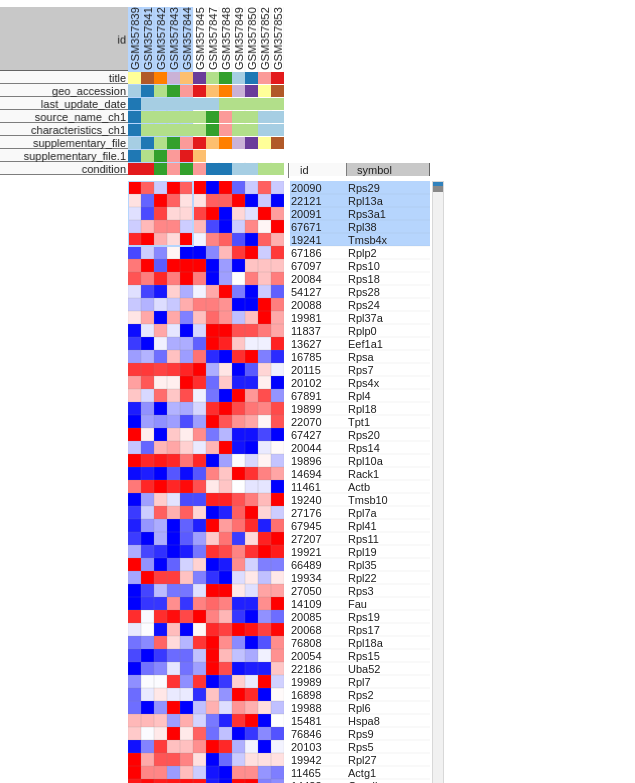
\includegraphics[scale=0.5]{heatmap14308.png}
  \caption{Визуализация матрицы GSE14308 в виде тепловой карты в веб-приложении Morpheus}
  \label{matrixvis}
\end{figure}


Также к основным методам анализа относятся:
\begin{itemize}
\item кластеризация:\begin{itemize}
\item иерархическая: метод упорядования данных таким образом, чтобы их можно было визуализировать в виде дерева (дендрограммы);
\item вероятностная: метод разбиения данных на несколько групп (кластеров);\end{itemize}
\item дифференциальная экспрессия: метод, позволяющий сравнивать поведение генов в разных условиях и искать закономерности;
\item метод главных компонент: метод для уменьшения размерности данных с наименьшей потерей информации. 
\end{itemize}

\section{Существующие решения для анализа экспрессии генов}
\subsection{R/Bioconductor}
\textbf{R} --- язык программирования для статистического анализа данных и работы с графикой~\cite{rproject}.

\textbf{Bioconductor} --- библиотека, содержащая в себе множество реализаций биоинформатических алгоритмов и методов обработки биологических данных на \emph{R}. Она постоянно обновляется, пополняется новыми библиотеками, модерируется сообществом~\cite{biobase}. \emph{R} и \emph{Bioconductor} очень популярны в биоинформатической среде ввиду предоставляемых возможностей.

Однако для качественного и полноценного анализа с помощью этих инструментов, нужно иметь навыки программирования на \emph{R}, что весьма неудобно для исследователей биологических специальностей.

\subsubsection{Biobase и ExpressionSet}
Необходимый минимум функций для работы с геномными данными содержится в \emph{R}-пакете \emph{Biobase}~\cite{biobase}.

Класс \texttt{ExpressionSet}~\cite{expressionset} также содержится в \emph{Biobase}. Он помогает представлять данные об экспрессии генов в удобном формате:
\begin{itemize}
\item \texttt{assayData} --- описание матрицы:\begin{itemize}
\item \texttt{features} --- количество генов;
\item \texttt{samples} --- количество образцов;
\item \texttt{exprs} --- числовая матрица экспрессии; \end{itemize}
\item \texttt{phenoData} --- аннотация к образцам:\begin{itemize}
\item \texttt{sampleNames} --- идентификаторы образцов;
\item \texttt{varLabels} --- названия характеристик;
\item \texttt{varMetadata} --- описание характеристик;
\item \texttt{pData} --- матрица характеристик;\end{itemize}
\item \texttt{featureData} --- аннотация к генам:\begin{itemize}
\item \texttt{featureNames} --- идентификаторы генов;
\item \texttt{fvarLabels} --- названия характеристик;
\item \texttt{fvarMetadata} --- описание характеристик;
\item \texttt{fData} --- матрица характеристик.\end{itemize}
\end{itemize}

Для доступа к каждому из элементов есть одноименная функция, что позволяет удобно взаимодействовать с экземплярами класса. Также многие из функций обработки данных в \emph{Bioconductor} и в \emph{Biobase} в частности завязаны на использование \texttt{ExpressionSet}.


\subsection{GENE-E}
\textbf{GENE-E} --- Платформа для анализа данных и визуального исследования данных, созданная на \emph{Java} и \emph{R}~\cite{genee}. Содержит в себе множество полезных для исследования инструментов: тепловые карты, кластеризацию, фильтрацию, построение графиков и т.д. Позволяет исследовать любые данные в виде матрицы. К тому же, содержит дополнительные инструменты для данных генетической экспрессии.

Недостатки:
\begin{itemize}
\item чтобы использовать, необходимо устанавливать на свой компьютер;
\item поддержка данного приложения прекратилась в связи с созданием \emph{morpheus.js}~\cite{morpheus};
\item не имеет открытого исходного кода, а только \emph{API} для взаимодействия и создания новых приложений на его основе.
\end{itemize}

\subsection{morpheus.js}
\textbf{Morpheus.js} --- веб-приложение для визуализации и анализа матриц от создателя \emph{GENE-E}~\cite{morpheus}. В отличие от предшественника, создано на \emph{JavaScript} и с открытым исходным кодом. Удобно для использования исследователями без навыков программирования и так же, как и \emph{GENE-E}, применимо к любым матрицам.

Недостатки:
\begin{itemize}
\item ограниченный набор функций, которых недостаточно для полноценного анализа;
\item для расширения биоинформатическими алгоритмами, не прибегая к дополнительным инструментам, требуется реализовывать их заново на \emph{JavaScript};
\end{itemize}

Далее будут описаны основные компоненты, классы и методы, реализованные в \emph{morpheus.js}, с которыми необходимо работать в случае расширения данного приложения.

\subsubsection{Чтение данных}
В \emph{morpheus.js} данные могут быть загружены из файла одним из следующих путей:
\begin{itemize}
\item Из компьютера;
\item По \emph{URL}-ссылке;
\item Из \emph{Dropbox}.
\end{itemize}

Допустимые форматы загружаемых файлов:
\begin{itemize}
\item \emph{txt}-файл с \emph{tab}-разделителями;
\item \emph{Excel}-таблица;
\item \emph{Mutation Annotation Format} (\emph{MAF})~\cite{maf};
\item \emph{Gene Cluster Text} (\emph{GCT})~\cite{gct};
\item \emph{Gene Matrix Transposed} (\emph{GMT})~\cite{gmt}.
\end{itemize}

Для каждого формата файла в исходном коде morpheus.js присутствует соответствующий обработчик данных.

Также, \emph{morpheus.js} предлагает набор предзагруженных данных из базы \emph{The Cancer Genome Atlas} (\emph{TCGA})~\cite{tcga}.

\subsubsection{Класс Dataset}
Одним из ключевых классов всего веб-приложения является класс \texttt{Dataset}. В каждом экземпляре этого класса хранится вся необходимая информация о данных, в которую входят:

\begin{itemize}
\item числовая матрица, характеризующая уровень экспрессии всех генов во всех образцах;
\item количество строк и столбцов в матрице;
\item аннотация к образцам, например:\begin{itemize}
\item пол, возраст, контактную информацию испытуемых, если образцы были взяты с людей;
\item есть или нет инфекция в данном образце;
    \item способ лечения;
    \item  контакты ответственного за взятие данного образца и пр.;\end{itemize}
\item аннотация к генам, например:\begin{itemize}
    \item идентификатор гена в том или ином стандарте;
    \item числовые характеристики гена (средний уровень экспрессии по образцам, номер кластера) и пр.\end{itemize}
\end{itemize}

Аннотация реализована в классе \texttt{MetadataModel}, который представляет собой не что иное, как набор именованных векторов с характеристиками. В каждом векторе хранятся:

\begin{itemize}
\item название;
\item формат (строка, число);
\item массив значений.
\end{itemize}

Для векторов так же предусмотрены утилиты для визуализации. Так, например, есть возможность показать аннотацию в виде текста и/или цветом, что удобно для категориальных характеристик. 

\subsubsection{Класс SlicedDatasetView}
Чаще всего во время работы программы экземпляры класса \texttt{Dataset} становятся обернуты в оболочку из \texttt{SlicedDatasetView}. Этот дополнительный класс дает возможность не пересоздавать каждый раз \texttt{Dataset}, а просто добавляет к данным информацию о том, какие индексы строк и столбцов выбраны и используются в данный момент и в каком порядке.

\subsubsection{Класс HeatMap}
Данный класс предназначен для визуализации данных, обернутых в класс \texttt{Dataset} или \texttt{SlicedDatasetView}. Он дает возможность выбирать, какая аннотация будет представлена на экране, цветовой код, выбирать строки и столбцы, с которыми будут работать те или иные инструменты.

\subsubsection{Класс DatasetUtil}
Класс \texttt{DatasetUtil} содержит в себе утилиты для обработки и чтения данных в \texttt{Dataset}:\begin{itemize}
\item обработка входных файлов с данными и отправка их на соответствующий класс чтения в зависимости от формата;
\item поиск по данным;
\item преобразование данных в \emph{JSON} и обратно.
\end{itemize}

\subsubsection{Реализованные методы}
В \emph{morpheus.js} имеются реализации следующих методов обработки и анализа данных:

\begin{itemize}
\item \texttt{Adjust} --- инструмент для корректировки данных:\begin{itemize}
    \item логарифмическое преобразование;
    \item обратное логарифмическое преобразование;
    \item квантиль-нормализация;
    \item z-тест;
    \item устойчивый Z-тест;\end{itemize}
\item \texttt{Collapse} --- инструмент, позволяющий агрегировать строки или столбцы с одинаковыми значениями с помощью функции: $\min$, $\max$, $mean$, $median$, $sum$, максимум 25-го и 75-го перцентилей;
\item \texttt{CalculatedAnnotation} --- добавление вычисленной аннотации для строк или столбцов;
\item \texttt{Similarity Matrix} --- построение матрицы соответствия строк или столбцов друг другу;
\item \texttt{Transpose} --- транспонирование матрицы;
\item \texttt{t-SNE} --- реализация алгоритма снижения размерности;
\item \texttt{ChartTool} --- построение графиков.
\end{itemize}

Также присутствуют фильтрация по строкам и столбцам и сортировка.

\subsection{ProjectX}
\textbf{ProjectX} --- веб-приложение, созданное в рамках выпускной квалификационной работы~\cite{projectx}, которое соединяло в себе возможности для веб-разработки, предоставляемые фреймворком \emph{Django} и методы из библиотеки \emph{Bioconductor} с помощью \emph{OpenCPU}.  Преимуществом данного приложения перед актуальным на тот момент \emph{GENE-E} была вопроизводимость исследований (на каждом этапе пользователь мог скачать исполняемый \emph{R}-код, эквивалентный коду, выполненному в сервисе), также он содержал в себе большее число методов анализа и обработки данных.

Недостатки:
\begin{itemize}
\item работа над проектом была завершена до того, как у него появились пользователи, так что оно осталось невостребованным.
\end{itemize}

\section{Использование R в веб-разработке}
Как было сказано ранее, \emph{R} удобно использовать для статистического анализа данных. Но чтобы использовать методы \emph{R} в веб-приложениях, возникает необходимость в дополнительных технологиях для интеграции инструментов веб-разработки и \emph{R}.

\subsection{Shiny}
\textbf{Shiny} --- фреймворк для создания веб-приложений, используя только язык \emph{R}~\cite{shiny}.
\subsection{OpenCPU}
\textbf{HTTP} (\emph{HyperText Transfer Protocol}) ---  протокол прикладного уровня передачи данных на основе технологии <<клиент-сервер>>~\cite{http}.

\textbf{HTTP API} - набор процедур и функций, вызов которых и возвращение их результа осуществляется посредством протокола \emph{HTTP}.

\textbf{RPC} (\emph{Remote Procedure Call}) --- класс технологий, позволяющих компьютерным программам вызывать функции или процедуры в другом адресном пространстве.

\textbf{Веб-сервер} --- сервер, принимающий \emph{HTTP}-запросы от клиентов, обычно веб-браузеров, и выдающий им \emph{HTTP}-ответы.

\textbf{OpenCPU} --- система для встроенных научных вычислений и воспроизводимых исследований, предоставляющая \emph{HTTP API} для вызова R-функций и взаимодействия с R-объектами с помощью \texttt{POST} и \texttt{GET} запросов~\cite{opencpu}.

\subsubsection{OpenCPU-сервер}\label{opencpuintro}
\emph{OpenCPU}-сервер можно запустить одним из следующих способов:
\begin{itemize}
\item однопользовательский сервер: сервер запускается из активной \emph{R}-сессии и предназначен в основном для разработки и локального использования. Такой сервер не поддерживает параллельных запросов, так как \emph{R}-сессии работают в одном потоке;
\item облачный сервер: этот сервер можно запустить на \emph{Ubuntu 16.04} и выше. Запуск и настройка облачного сервера осуществляется с помощью \emph{Apache} или \emph{Nginx}. В отличие от однопользовательского сервера, здесь поддерживаются параллельные запросы и настройка безопасности.
\end{itemize}

Однопользовательский сервер в большинстве случаев работает значительно быстрее, чем облачный, так как последний управляется с помощью \emph{rApache}~\cite{rapache}, что добавляет удобства в использовании, но замедляет доступ к серверу. Первым же можно пользоваться как многопользовательским, используя несколько экземпляров сервера, доступ к которым осуществляется с помощью \emph{Apache} и балансировщика, который тот предоставляет.

\subsubsection{OpenCPU API}
Входной точкой \emph{API} является \texttt{/ocpu/}.
\texttt{GET}-запрос используется для получения некоторого ресурса, а \texttt{POST}-запрос используется для \emph{RPC}. На таблице~\ref{ocpu_api} можно увидеть более подробное описание запросов.

\begin{table}[!h]
  \small
\caption{Запросы к \emph{OpenCPU}-серверу, их аргументы и действия}\label{ocpu_api}
\centering
\begin{tabu} to \textwidth {| l | L | K | X |}
  \hline
Запрос        & Действие          & Аргументы                    & Пример                                 \\\hline 
\texttt{GET}  & посмотреть объект & формат представления объекта & GET /ocpu/library/MASS/R/cats/json     \\\hline
\texttt{POST} & вызвать функцию   & аргументы функции            & POST /ocpu/library/stats/R/rnorm       \\\hline
\texttt{GET}  & прочитать файл    & -                            & GET /ocpu/library/MASS/NEWS            \\\hline
\texttt{POST} & запустить скрипт  & аргументы запуска скрипта    & POST /ocpu/library/MASS?scripts/ch01.R \\\hline
\end{tabu}
\end{table}

На \emph{OpenCPU}-сервере могут быть доступны:
\begin{itemize}
\item библиотеки и содержащиеся в них пакеты: \texttt{/ocpu/library/{pkgname}/};
\item пакеты из \emph{git}-репозиториев: \texttt{/ocpu/apps/{gituser}/{reponame}/};
\item пакеты, установленные в домашней директории \emph{Linux}-пользователя: \texttt{/ocpu/user/{username}/library/{pkgname}/};
\item временные сессии, содержащие вывод от запуска функции или скрипта: \texttt{/ocpu/tmp/{key}/}.
\end{itemize}

\subsubsection{Opencpu.js}
Так как зачастую \emph{OpenCPU} используется разработчиками для использования \emph{R} в веб-приложениях для анализа и визуализации данных, для удобной интеграции \emph{JavaScript} и \emph{R} существует библиотека \textit{opencpu.js}, которая реалазует \emph{RPC}-вызовы по принципу \emph{Asynchronous JavaScript and XML} (\emph{Ajax}~\cite{ajax}). Таким образом запросы обрабатываются в фоновом режиме, тем самым не замедляя работу графического интерфейса и вычислений, осуществляемых на стороне клиента.

В данной библиотеке реализован класс \texttt{Session}, содержащий в себе ключ сессии, адреса на ссылки, файлы и переменные, существующие внутри сессии.

Для подключения к \emph{R}-пакету на \emph{OpenCPU}-сервере удобно использовать код, представленный на листинге~\ref{connect}. Для успешного подключения \emph{R}-пакет должен быть предварительно установлен на \emph{host}-машину, на которой располагается сервер. 

\begin{lstlisting}[float=!h,caption={Подключение к \emph{R}-пакету},label={connect}]
  ocpu.seturl("//hostname/ocpu/library/{pkgname}/R");
\end{lstlisting}
После этого можно вызывать и запускать функции, содержащиеся в данном \emph{R}-пакете, например, как в листинге~\ref{call.example}.

\begin{lstlisting}[float=!h,caption={Шаблон вызова \emph{R}-функции из \emph{JavaScript}},label={call.example},language=JavaScript]
  var req = ocpu.rpc("function.name", arguments, callback(session) {
    \\ Handling result
  });
\end{lstlisting}

\section{Инфраструктура}
\subsection{Docker}
\textbf{Docker} --- программное обеспечение для автоматизации запуска и внедрения приложений внутри контейнеров~\cite{docker}.

Для дальнейшего описания данного инструмента введем несколько определений.

\textit{Образ} --- отдельный исполняемый пакет, включающий себя все необходимое для запуска единицы программного обеспечения, в том числе исходный код, библиотеки, переменные окружения, конфигурационные файлы. Зачастую образ построен на основе другого образа с дополнительной конфигураций. Образ компилируется по \textit{Dockerfile}, каждая команда в котором соответствует новому слою. При перекомпиляции обновляются только те слои, которые изменились. 

\textit{Контейнер} --- запущенный экземпляр образа. Контейнер обычно исполняется изолированно от окружения, имея доступ к файлам или портам хост-системы только при наличии соответствующей конфигурации.

В отличие от виртуальных машин, которые запускают гостевую операционную систему в каждом экземпляре, контейнеры могут разделять общее ядро, и вся информация, которая должна быть в контейнере, это исполняемый процесс и его зависимости. Исполняемые процессы из контейнеров работают как нативные процессы, и могут управляться по отдельности. 

Для контроля версий и хранения образов в открытом доступе используется \emph{Docker Hub}~\cite{dhub}. В этом хранилище можно как добавлять репозитории, управляемые вручную, так и поддерживать автоматические сборки (\textit{Automated Build}), которые привязаны к репозиториям на в популярных системах контроля версий: GitHub~\cite{github} и Bitbucket~\cite{bitbucket}.
\subsection{Apache}
\textbf{Apache HTTP Server Project} --- устойчивый, полностью открытый \emph{HTTP}-сервер~\cite{apache}.

\emph{Apache} позволяет конфигурировать веб-сервисы, переадресацию, балансировку нескольких экземпляров серверов. 
\section{Форматы сериализации данных}
\subsection{JSON}
\textbf{JSON} --- текстовый формат представления данных, основанный на \emph{JavaScript}, который, среди прочих достоинств, легко читается человеком.

\emph{JSON}-текст представляет собой одну из следущих структур:\begin{itemize}
\item пара \textit{ключ}: \textit{значение}, где ключом может быть только регистрозависимая строка, а в качестве значения может выступата массив, число, строка, литералы или другой \emph{JSON}-объект;
\item набор значений.
\end{itemize}

\subsection{Protocol Buffers}
\textbf{Protocol Buffers (Protobuf)} --- гибкий, универсальный и автоматизированный механизм для сериализации структурированных данных~\cite{protobuf}.

Структура информации задается с помощью \texttt{*.proto}-файлов в форме сообщений (\texttt{message}).

\emph{ProtoBuf}-формат не является человекочитаемым, данные хранятся в двоичном формате. Для десериализации и дальнейшего чтения необходим соответствующий \texttt{*.proto}-файл. Файл с форматом компилируется соответствующим выбранному языку программирования компилятором, таким образом будет создан класс доступа к данным. С помощью этого класса уже можно сериализовать/десериализовать данные, получать данные с помощью \texttt{get}/\texttt{set}-методов и пр.

\section{Открытые источники данных экспрессии генов}
\subsection{Gene Expression Omnibus}\label{geointro}
\textbf{Gene Expression Omnibus (GEO)} --- международный публичный репозиторий, агрегирующий и распространяющий различные формы геномных данных от исследовательского сообщества~\cite{geo}.

\emph{GEO} предоставляет устойчивую базу данных для эффективного хранения геномных данных, содержит их в качественно аннотированном формате и дает возможность удобно как добавлять новые данные для публикации, так и запрашивать интересующие данные для исследований.

В \emph{GEO} содержатся следующие типы и форматы данных:
\begin{itemize}
\item информация о платформе, на которой производилось секвенирование генов (\emph{Platform records}): \texttt{GPLxxx};
\item информация об образцах и условиях, в которых производились исследования этих образцов (\emph{Sample records}): \texttt{GSMxxx};
\item информация о непосредственно исследованиях, полученные данные и выводы (\emph{Series records}): \texttt{GSExxx}.
\item обработанная и подготовленная для дальнейшего статистического анализа \emph{GEO}-кураторами информация об исследованиях (\emph(DataSet records)): \texttt{GDSxxx}.
\end{itemize}

В библиотеке \emph{Bioconductor} есть \emph{R}-пакет \emph{GEOquery} для удобной загрузки данных из \emph{GEO}~\cite{geoquery}.
\subsection{The Cancer Genome Atlas}
\textbf{The Cancer Genome Atlas (TCGA)} --- проект, нацеленный на систематизацию данных о генетических мутациях, приводящих к возникновению рака. На данный момент участниками проекта отсеквенировано и проанализировано 33 вида рака~\cite{tcga}.

\section{Постановка задачи}
Рассмотрев существующие решения для анализа экспрессии генов и инструментов, которые могли бы пригодиться для будущих решений, можно сформулировать цель и основные задачи данной работы

\subsection{Цель работы}
Целью работы является создание веб-приложения, интегрирующего существующие возможности веб-приложения \emph{morpheus.js} и методы анализа, реализованные в \emph{Bioconductor}.

\subsection{Основные задачи}
Для достижения поставленной цели были сформулированы следующие задачи:
\begin{enumerate}
\item разработать способ взаимодействия между \emph{js}-клиентом и \emph{R} и встроить его в \emph{morpheus.js}, чтобы избежать реализации с нуля уже существующих алгоритмов;
\item реализовать графический интерфейс в \emph{js}-клиенте и серверную реализацию в \emph{R}-пакете;
\item соединить все составляющие в одном веб-приложении \emph{phantasus};
\item запустить веб-приложение в открытый доступ для исследователей.
\end{enumerate}

\subsection{Требования к веб-приложению phantasus}
\subsubsection{Доступность}
Необходимо, чтобы веб-приложение \emph{phantasus} было доступно для исследователей независимо от их местоположения и времени суток. Варианты действий:

\begin{enumerate}
\item сделать его доступным по определенному веб-адресу, и тогда пользователь сможет продолжать исследования из любой точки, где есть подключение к интернету;
\item предоставить возможность запускать приложение локально, например, с помощью \emph{Docker} или внутри \emph{R}.
\end{enumerate}

\subsubsection{Возможность дальнейшего расширения функционала}
Как уже было сказано выше, библиотека \emph{Bioconductor} постоянно обновляется и пополняется новыми алгоритмами, а исследователи находят новые методы для анализа экспрессии генов, так что необходимо не только реализовать дополнительные методы, но также отладить и описать алгоритм действий для добавления новых.

\chapterconclusion
В данной главе были введены понятия биоинформатики и анализа экспрессии генов, обозначена цель работы и задачи, выполнение которых необходимо для ее достижения, представлены существующие решения с их достоинствами и недостатками, а также перечислен ряд инструментов, которые могут быть использованы для решения поставленных задач работы.

\finishrelatedwork

\chapter{Архитектура проекта phantasus}
В этой главе будет рассмотрена архитектура проекта \emph{phantasus}, общая схема, ключевые компоненты и их взаимодействие между ними. Также будут описаны сопутствующие инструменты и их предназначение в системе, и ключевые для архитектуры выдержки из исходного кода.

\section{Общая схема}
Проект \emph{phantasus} состоит из следующих компонент:\begin{itemize}
\item клиентская сторона проекта: \emph{phantasus.js} --- модифицированный \emph{morpheus.js}, дополненный интерфейсами для новых инструментов, поддержкой \texttt{ExpressionSet} и сериализации в \emph{ProtoBuf};
\item серверная сторона проекта: \emph{R}-пакет \emph{phantasus} --- пакет, включающий в себя вычисления и реализации новых инструментов.\end{itemize}

Общую схему взаимодействия можно увидеть на диаграмме~\ref{scheme}.

\begin{figure}[!h]
  \caption{Общая схема проекта \emph{phantasus}}
  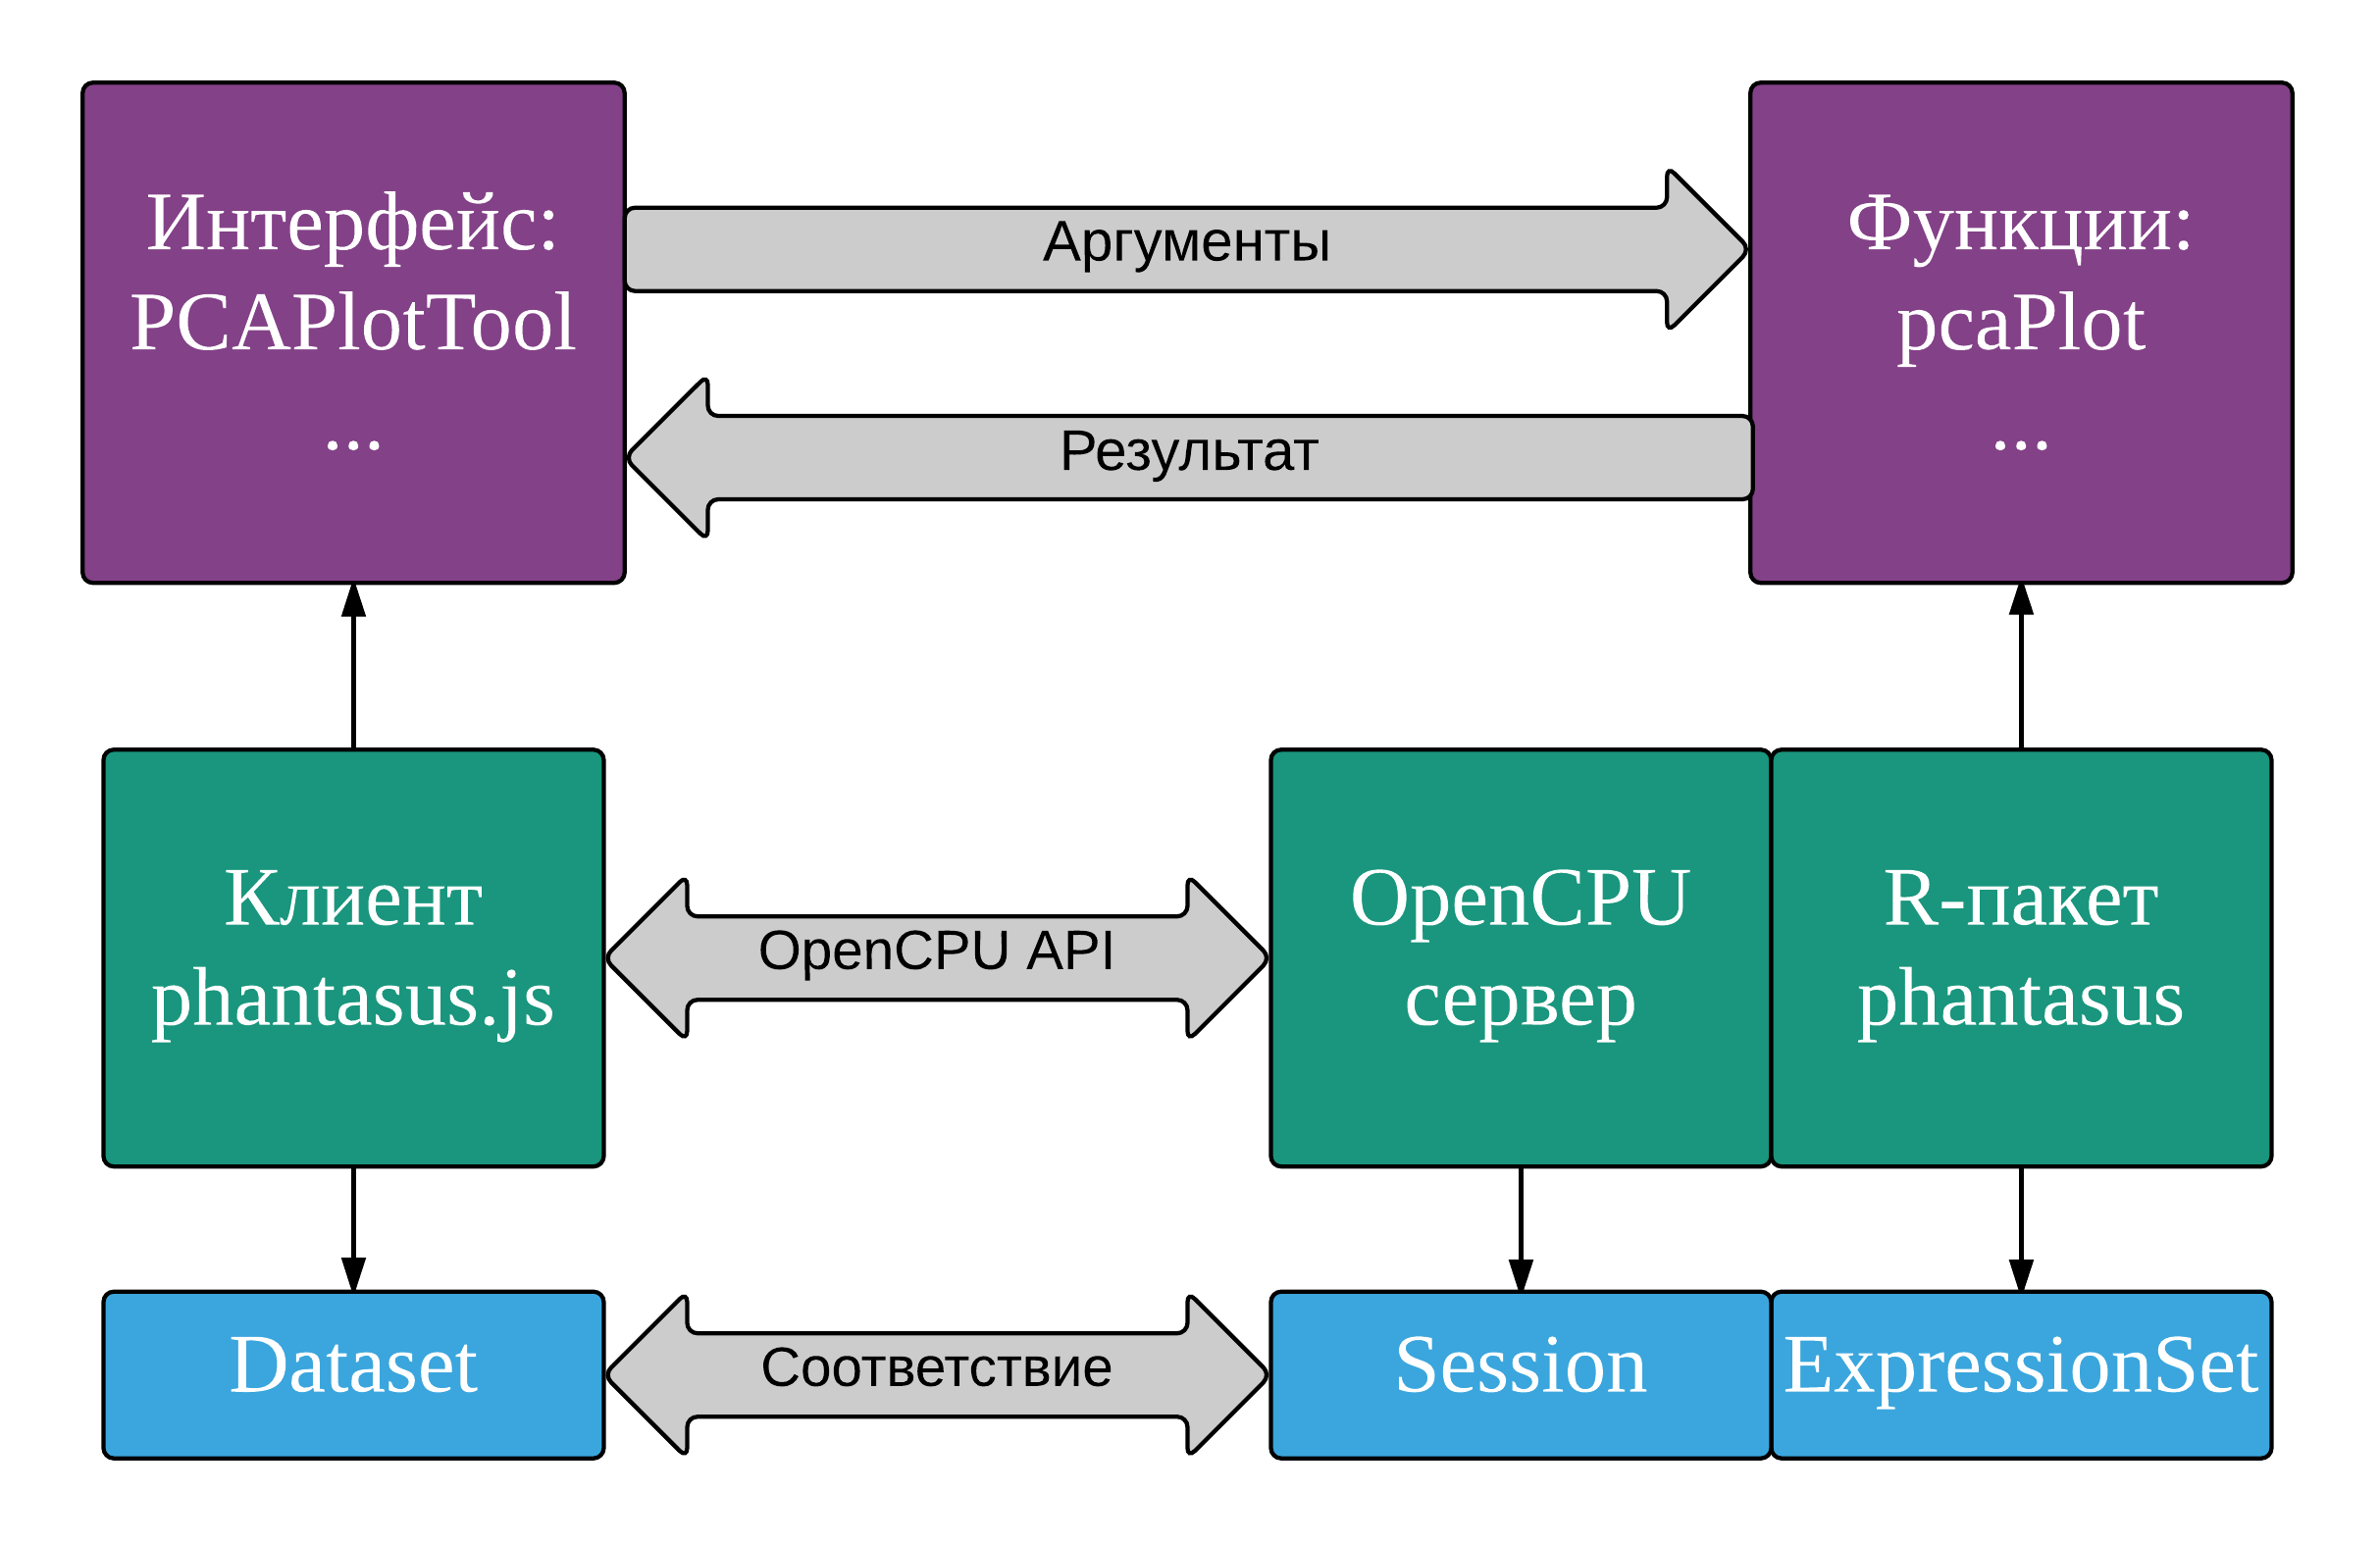
\includegraphics[scale=0.8]{scheme_phantasus.png}
  \label{scheme}
\end{figure}

\section{Взаимодействие между клиентом и сервером}
Все инструменты, реализованные в проекте, имеют две компоненты:\begin{itemize}
\item графический интерфейс в \emph{phantasus.js};
\item вычислительную реализацию в \emph{R}-пакете \emph{phantasus}.
\end{itemize}

Соответственно, для связи этих компонент необходим своеобразный мост между клиентом, написанном на \emph{JavaScript}, и функциями, написанными на \emph{R}. В качестве такого моста используется описанный в обзоре \emph{OpenCPU}.

Помимо наличия моста также необходимо, чтобы общение между клиентом и сервером происходило достаточно быстро, что приводит к потребности в дополнительной сериализации сообщений. В проекте для этого используется протокол \emph{ProtoBuf}.
В данном разделе будет подробно описано об использовании данных технологий при реализации взаимодействия между клиентом и сервером.
\subsection{OpenCPU}
Как было сказано выше, \emph{OpenCPU} используется для связи между \emph{JavaScript}-клиентом и \emph{R}-функциями.

\subsubsection{Использование OpenCPU со стороны клиента}\label{functioncallalgo}
Как было сказано в обзоре, для удобной интеграции \emph{JavaScript} и \emph{R} существует \emph{JavaScript}-библиотека \emph{opencpu.js}, в которой реализованы \emph{RPC}-вызовы. С помощью этой библиотеки в проекте реализована взаимосвязь между графическими интерфейсом инструментов и соответствующих функций из \emph{R}-пакета.

Каждый из инструментов, реализованных в \emph{phantasus.js} действует по следующему принципу:\begin{enumerate}
\item обработка аргументов, полученных в интерфейсе;
\item подготовка данных и аргументов к отправке на сервер;
\item \emph{RPC}-вызов функции, как на листинге~\ref{call.example};
\item обработка содержащегося в полученной сессии результата в виде глобальной переменной, ответа функции или сохраненного в сессии файла;
\item передача ответа в интерфейс.
\end{enumerate}

\subsubsection{Использование OpenCPU со стороны R-пакета}
Со стороны \emph{R}-функций никаким специальным образом не обозначается, что результат работы будет передан именно в \emph{JavaScript}-клиент, все реализованные функции достаточно универсальны.
Функция возвращает результат, в некоторых случаях дополнительно сохраняя его в файл или глобальную переменную, что в дальнейшем использует клиент, который заранее знает, в каком формате получит ответ. 

\subsection{Protocol Buffers}
\emph{OpenCPU API} поддерживает передачу сообщений в \emph{ProtoBuf}-формате. Однако, \emph{JavaScript}-библиотека не предусматривает такой возможности, так что в процессе работы над проектом была добавлена сериализация данных в \emph{ProtoBuf} на стороне клиента и поддержка сериализованных сообщений в \emph{opencpu.js}. 
\subsubsection{Сериализация данных со стороны клиента --- protobuf.js}
Чаще всего обрабатываемые матрицы содержат от 10000 до 40000 строк и от 12 до 40 столбцов. Соответственно, пересылать их между клиентом и сервером в \emph{JSON}-формате слишком долго.

Как было сказано в обзоре, технология \emph{Protocol Buffers} позволяет лучше сериализовать данные, чтобы уменьшить размер пересылаемого пакета.

К сожалению, \emph{Google Developers} официально поддерживают только \emph{Java}, \emph{Python}, \emph{C++}, \emph{Go}, \emph{Objective-C}, \emph{Ruby}, \emph{JavaNano} и \emph{C\#}. Для \emph{JavaScript} сообщество создает поддержку самостоятельно. После анализа существующих решений, было решено выбрать библиотеку \emph{ProtoBuf.js}~\cite{protobufjs}.

Данная библиотека реализует класс \texttt{Builder}, который компилируется из \texttt{*.proto}-файлов и позволяет получить доступ к сериализованным данным. С помощью экземпляра данного класса можно закодировать соответствующий \emph{JSON}-объект в \texttt{Uint8Array}, чтобы после переслать его в сжатом виде на сервер.

Для преобразования экземпляров классов \texttt{Dataset} и \texttt{SlicedDatasetView}, которые были представлены в обзоре приложения \emph{morpheus.js}, в сериализованнный \texttt{Uint8Array} используется протокол, описанный в приложении~\ref{proto}. Данный протокол используется также в \emph{R}-пакете \emph{protolite}~\cite{protolite}, с помощью которого данные десериализуются на сервере.

Таким образом в класс \texttt{DatasetUtil} была добавлена утилита, сериализующая \texttt{Dataset}, которая используется перед отправкой данных на сервер, и десериализующая результат работы \emph{R}-функций, если те сохраняют результат в бинарном файле. 
\subsubsection{Сериализация данных со стороны сервера --- protolite}
Внутри \emph{R}-функций нет необходимости вручную явно десериализовавать входные данные, так как \emph{OpenCPU} автоматически разбирает аргументы до входа в функцию.

Однако, если функция возвращает матрицы больших размеров, используется \emph{R}-пакет \emph{protolite}~\cite{protolite} для сериализации результата работы, который после сериализованный записывается в бинарный файл. В дальнейшем этот файл считывается клиентом из директории возвращенной временной сессии. 

\section{Поддержка ExpressionSet}
Как было сказано ранее, а также продемонстрировано на схеме~\ref{scheme}, в ходе работы приложения постоянно поддерживается соответствие между экземпляром класса \texttt{Dataset} на клиенте и экземпляром класса \texttt{ExpressionSet} на сервере. В данном разделе будет подробнее разобрана реализация данного соответствие.
\subsection{Поддержка ExpressionSet на стороне клиента}
В \emph{phantasus.js} в Dataset добавлено дополнительное поле \texttt{esSession}, в котором находится объект класса \texttt{Promise} для асинхронного обновления ключа сессии в этом поле.

При загрузке или обновлении \texttt{Dataset} осуществляется следующий ряд действий:
\begin{enumerate}
\item в поле \texttt{dataset.esSession} записывается экземпляр класса \texttt{Promise}, который позволяет продолжать загрузку данных в фоновом режиме, а также ждать, когда данные будут обработаны прежде чем запускать функции использующие \texttt{ExpressionSet} в качестве аргумента (\texttt{pcaPlot}, \texttt{kmeans}, \texttt{limma}). При создании \texttt{Promise} в аргументах указывается две функции: \texttt{reject} и \texttt{resolve};
\item актуальное содержимое экземпляра класса \texttt{Dataset} вместе с матрицей и аннотацией сериализуется в \emph{ProtoBuf} по протоколу, описанному в приложении~\ref{proto};
\item с помощью \emph{opencpu.js} отправляется \emph{RPC} за функцией \texttt{createES} с аргументом в виде сериализованных данных;
\item данные поступают на сервер, десериализуются там автоматически и функция \texttt{createES} создает \texttt{ExpressionSet}, являющийся копией \texttt{Dataset} из клиента;
\item функция \texttt{createES} объявляет данный \texttt{ExpressionSet} глобальной переменной, таким образом имеется доступ к этому объекту по \emph{API-entrypoint} \texttt{/ocpu/tmp/{key}/R/es};
\item по завершении \emph{RPC} получает ключ временной сессии, содержащий созданный \texttt{ExpressionSet} и завершает \texttt{Promise} с \texttt{resolve(session)};
\item если во время одного из этапов произошла ошибка, то \texttt{Promise} завершается с \texttt{reject(error)} с текстом ошибки.
\end{enumerate}

\subsection{Создание ExpressionSet из внешних данных на стороне сервера} \label{createESsection}
В начале работы с \emph{phantasus} необходимо загрузить данные. Если данные загружены из файла, то они будут сначала обработаны на клиенте, а после пересланы на сервер для создания \emph{ExpressionSet} из них с помощью кода на листинге~\ref{createES}.

Функция \texttt{createES} принимает следующие аргументы:\begin{itemize}
\item \texttt{data} --- непосредственно матрица экспрессии;
\item \texttt{pData} --- аннотация к образцам;
\item \texttt{varLabels} --- названия характеристик описания образцов;
\item \texttt{fData} --- аннотация к генам;
\item \texttt{fvarLabels} --- названия характеристик описания генов.
\end{itemize}

\begin{lstlisting}[float=!h,caption={Функция создания ExpressionSet из исходных данных},label={createES},language=R]
createES <- function(data, pData, varLabels, fData, fvarLabels) {
  exprs <- t(data)
  phenoData <- AnnotatedDataFrame(data.frame(pData))
  varLabels(phenoData) <- varLabels
  
  featureData <- AnnotatedDataFrame(data.frame(fData))
  varLabels(featureData) <- fvarLabels
 
  es <- ExpressionSet(assayData = exprs, phenoData=phenoData, featureData = featureData)
  assign("es", es, envir = parent.frame())
  es
}
\end{lstlisting}

По завершении функция отправляет \texttt{es} в глобальные переменные, чтобы созданный \texttt{ExpressionSet} был доступен по адресу: \texttt{/ocpu/tmp/{key}/R/es}. Таким образом, получив ключ данной сессии, можно иметь доступ и к \texttt{ExpressionSet}, находящемуся в ней.

Ключ сессии обновляется каждый раз при изменении \texttt{Dataset} в \emph{phantasus.js}. Чаще всего изменения происходят в результате работы одного из следующих инструментов: \texttt{Adjust}, \texttt{Collapse}, \texttt{new HeatMap}, \texttt{Transpose}. Изменные данные, точно так же ,как и новые, пересылаются на сервер и ключ сессии обновляется в поле \texttt{esSession} в \texttt{Dataset}.

\section{Способы визуализации}
В данном разделе будут показаны достоинства и недостатки различных способов визуализации, а также применимость в различных ситуациях. 
\subsection{Отрисовка графиков на стороне сервера}
Первый вариант визуализации графиков и схем состоит в отрисовке их там же, где и происходит вычисление всех необходимых для них данных, то есть на сервере внутри \emph{R}-функции. Данный способ подразумевает отрисовку и сохранение изображений в виде \emph{png} или \emph{svg}-файла, который сохраняется внутри временной \emph{OpenCPU}-сессии. Клиент после забирает из сессии изображение и показывает в графическом интерфейсе приложения.

Достойнства:\begin{itemize}
\item возможность пользоваться проверенными \emph{R}-пакетами для визуализации, например, \emph{ggplot2}~\cite{ggplot2};
\item файл можно переиспользовать при необходимости, нужно знать только ключ сессии, где он находится.
\end{itemize}

Однако таким образом можно использовать только статичные изображения.

\subsection{Визуализация на стороне клиента}
Для отображения интерактивных графиков удобно использовать библиотеку \emph{plotly.js}~\cite{plotly}, которая предоставляет \emph{API}, где описание графика строится в \emph{JSON}-формате.
Таким образом можно строить интерактивные изображения, переложить всю работу по визуализации с сервера на клиент.

Именно этот способ на данный момент используется в проекте, подробнее об инструменте будет рассказано в главе~\ref{implementation}.

\chapterconclusion
В данной главе были рассмотрены основные составляющие проекта:
\begin{itemize}
\item \emph{phantasus.js} --- расширенный \emph{morpheus.js};
\item \emph{R}-пакет \emph{phantasus} --- \emph{R}-пакет, содержащий в себе серверные реализации всех добавленных методов и инструментов.
\end{itemize}

Также были представлены следующие подробности архитектуры проекта:\begin{itemize}
\item общая схема всего проекта, где показаны компоненты и связи между ними;
\item способ взаимодействия между компонентами с помощью \emph{OpenCPU};
\item сериализация данных в \emph{ProtoBuf} на стороне клиента и на стороне сервера;
\item поддержка \texttt{ExpressionSet};
\item способы визуализации.
\end{itemize}


\chapter{Реализация и использование}\label{implementation}
В этой главе будут подробно описаны реализованные методы анализа в проекте \emph{phantasus}, их реализация на стороне сервера и на стороне клиента, будет рассказано о способах запуска приложения и другие инфраструктурные подробности.
\section{Реализованные методы анализа экспрессии}
В ходе работы над проектом были реализованы следующие функции и методы анализа экспрессии:\begin{itemize}
\item \texttt{loadGEO} --- загрузка и визуализация данных из \emph{Gene Expression Omnibus};
\item \texttt{pcaPlot} --- реализация метода главных компонент и визуализация результата;
\item \texttt{kmeans} --- реализация кластеризации методом \emph{kmeans};
\item \texttt{limmaAnalysis} --- анализ дифференциальной экспрессии для сравнения образцов. \end{itemize}

В этом разделе будут один за другим описаны все вышеперечисленные методы.

\subsection{Загрузка данных из GEO}
В разделе~\ref{geointro} обзора были описаны форматы данных в репозитории \emph{Gene Expression Omnibus}.
В \emph{phantasus} загрузка данных из \emph{GEO} осуществляется следующим образом:
\begin{enumerate}
\item функция \texttt{loadGEO} принимает на вход идентификатор \texttt{GEO};
\item в зависимости от его вида (\emph{GSE} или \emph{GDS}) запускаются дополнительные функции (\texttt{getGSE} на листинге~\ref{getGSE} и \texttt{getGDS} на листинге~\ref{getGDS});
\item в каждой из двух функций с помощью \texttt{GEOquery::getGEO} загружаются данные с аннотацией (или подгружаются из кэша, если он указан или если их уже загружали);
\item результат обрабатывается, создается \texttt{ExpressionSet} и отправляется в глобальные переменные;
\item в файл записываются сериализованные в \emph{ProtoBuf} данные, в том же формате, что и при создании \texttt{ExpressionSet} из внешних данных (смотри раздел~\ref{createESsection}), которые после считает и обработает клиент.
\end{enumerate}
\begin{lstlisting}[float=!h,caption={Загрузка данных типа GSE из Gene Expression Omnibus},label={getGSE},language=R]
getGSE <- function(name, destdir = tempdir()) {
  es <- getGEO(name, AnnotGPL = T, destdir = destdir)[[1]]
  featureData(es) <- featureData(es)[,grepl("symbol", fvarLabels(es), ignore.case = T)]
  phenoData(es) <- phenoData(es)[,grepl("characteristics", varLabels(es), ignore.case = T)
                                  | (varLabels(es) %in% c("title", "id", "geo_accession"))]
  chr <- varLabels(es)[grepl("characteristics", varLabels(es), ignore.case = T)]
  take <- function(x, n) {
    sapply(x, function(x) { x[[n]] })
  }
  rename <- function(prevName, x) {
    splitted <- strsplit(x, ": ")
    sumlength <- sum(sapply(as.vector(splitted), length))
    if (sumlength != 2 * length(x)) {
       return(list(name = prevName, x = x))
    }
    splittedFirst <- unique(take(splitted, 1))
    if (length(splittedFirst) == 1) {
       res = list(name = splittedFirst[1], x = take(splitted, 2))
    }
    else {
       res = list(name = prevName, x = x)
    }
    res
  }
  renamed <- lapply(chr, function(x) { rename(x, as.vector(pData(es)[,x])) })
  phenoData(es) <- phenoData(es)[, !(varLabels(es) %in% chr)]
  pData(es)[,take(renamed,1)] <- take(renamed,2)
  es
}
\end{lstlisting}

\begin{lstlisting}[float=!h,caption={Загрузка данных типа GDS из Gene Expression Omnibus},label={getGDS},language=R]
 getGDS <- function(name, destdir = tempdir()) {
  l <- getGEO(name, destdir = destdir)
  table <- slot(l, 'dataTable') # extracting all useful information on dataset
  data <- Table(table)  # extracting table ID_REF | IDENTIFIER/SAMPLE | SAMPLE1 | ...
  columnsMeta <- Columns(table) # phenoData
  sampleNames <- as.vector(columnsMeta[["sample"]])
  rownames <- as.vector(data[["ID_REF"]])
  symbol <- as.vector(data[["IDENTIFIER"]])
  data <- data[,sampleNames] # expression data
  exprs <- as.matrix(data)
  row.names(exprs) <- rownames
  row.names(columnsMeta) <- sampleNames
  # columnsMeta <- columnsMeta[,!(colnames(columnsMeta) %in% c('sample'))] 
  pData <- AnnotatedDataFrame(data.frame(columnsMeta, check.names = F))
  fData <- data.frame(matrix(symbol, nrow(exprs), 1));
  colnames(fData) <- "symbol"
  fData <- AnnotatedDataFrame(fData)
  featureNames(fData) <- rownames
  ExpressionSet(assayData = exprs, phenoData = pData, featureData = fData)
}
\end{lstlisting}

Основной код загрузки и дополнительные утилиты к нему можно увидеть на листинге~\ref{loadGEO}.

\begin{lstlisting}[float=!h,caption={Загрузка данных из Gene Expression Omnibus},label={loadGEO},language=R]
loadGEO <- function(name, type = NA) {
  es <- getES(name, type, destdir = "/var/phantasus/cache")
  assign("es", es, envir = parent.frame())
  data <- as.matrix(exprs(es)); colnames(data) <- NULL; row.names(data) <- NULL

  pdata <- as.matrix(pData(es)); colnames(pdata) <- NULL; row.names(pdata) <- NULL

  participants <- colnames(es)
  rownames <- rownames(es)

  fdata <- as.matrix(fData(es))
  colnames(fdata) <- NULL
  row.names(fdata) <- NULL

  res <- list(data = data, pdata = pdata,
              fdata = fdata, rownames = rownames,
              colMetaNames = varLabels(phenoData(es)),
              rowMetaNames = varLabels(featureData(es)))

  f <- tempfile(pattern = "gse", tmpdir = getwd(), fileext = ".bin")
  writeBin(protolite::serialize_pb(res), f)
  f
}
getES <- function(name, type = NA, destdir = tempdir()) {
  if (is.na(type)) {
     type = substr(name, 1, 3)
  }
  if (type == 'GSE') {
    es <- getGSE(name, destdir)
  }
  else if (type == 'GDS') {
    es <- getGDS(name, destdir)
  }
  else {
    stop("Incorrect name or type of the dataset")
  } 
  es
}
\end{lstlisting}


\subsection{Метод главных компонент и визуализация его результата}
Данный инструмент предназначен для построения графиков в соответствие с методом главных компонент.
В качестве аргументов на вход к инструменту подается:
\begin{itemize}
\item номера образцов для сравнения;
\item категориальная аннотация для различения точек по цвету (если не указана, то стандартный цвет);
\item числовая аннотация для различения точек по размеру (если не указана, то стандартный размер);
\item аннотация для подписей к точкам (если не указана, то без подписи);
\item функция замены \texttt{NA} в данных при вычислении матрицы \emph{PCA} (\texttt{mean} или \texttt{median}).
\end{itemize}

\begin{figure}[h]
  \caption{Инструмент \texttt{PcaPlotTool} и отрисованный график по данным GSE14308}
  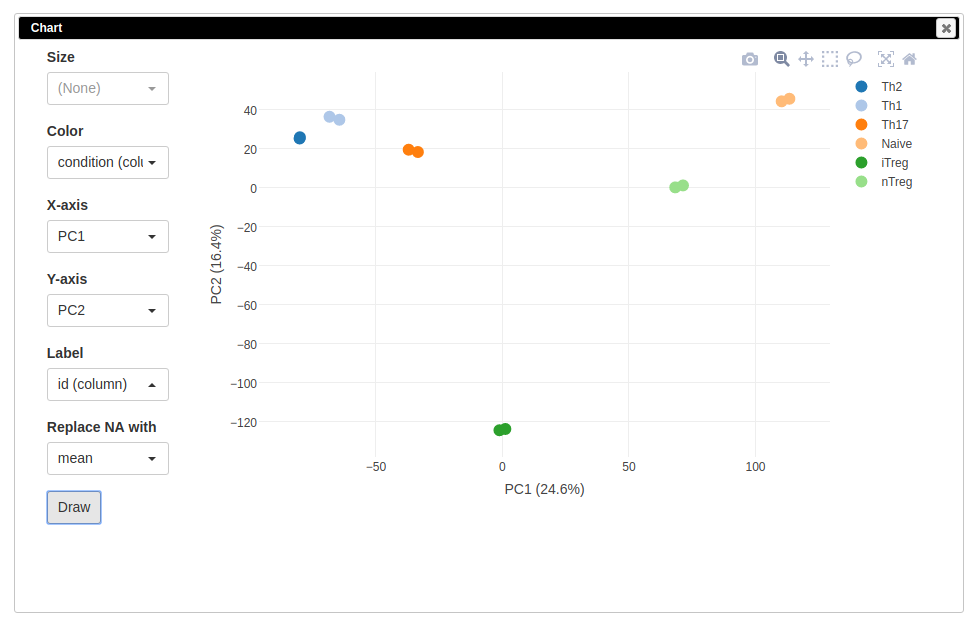
\includegraphics[scale=0.4]{plotexample.png}
  \label{plotexample}
\end{figure}

Далее по алгоритму, описанному в разделе~\ref{functioncallalgo}, на \emph{OpenCPU}-сервер отправляется \emph{RPC}-вызов с аргументами: ключ сессии, содержащий актуальный \texttt{ExpressionSet}, и функция замены \texttt{NA}.

Данные аргументы приходят на вход к функции \texttt{pcaPlot}, реализованной в \emph{R}-пакете \emph{phantasus}, код которой можно увидеть на листинге~\ref{pcaPlot}. Предварительно все \texttt{NA}-значения заменяются в соответствии с переданной функцией, если этого не сделать, то дальнейшие вычисления будут невозможны. Матрица экспрессии из входного \emph{ExpressionSet} передается в стандартную функцию \texttt{prcomp} из \emph{R}-пакета \emph{stats}~\cite{stats}, которая и вычисляет результирующую матрицу.
\begin{lstlisting}[float=!h,caption={Вычисление матрицы главных компонент},label={pcaPlot},language=R]
  pcaPlot <- function(es, rows=c(), columns = c(), replacena = "mean") {
  rows <- getIndicesVector(rows, nrow(exprs(es)))
  columns <- getIndicesVector(columns, ncol(exprs(es)))
  data <- data.frame(exprs(es))[rows, columns]

  ind <- which(is.na(data), arr.ind = T)
  if (nrow(ind) > 0) {
    data[ind] <- apply(data, 1, replacena, na.rm = T)[ind[,1]]
  }
  ind1 <- which(!is.nan(as.matrix(data)), arr.ind = T)
  left.rows <- unique(ind1[,"row"])
  data <- data[left.rows,]
  data <- t(data)

  pca <- prcomp(data)
  explained <- (pca$sdev)^2 / sum(pca$sdev^2)

  xs <- sprintf("PC%s", seq_along(explained))
  xlabs <- sprintf("%s (%.1f%%)", xs, explained * 100)

  pca.res <- as.matrix(pca$x); colnames(pca.res) <- NULL; row.names(pca.res) <- NULL
  return(jsonlite::toJSON(list(pca = t(pca.res), xlabs=xlabs)))
}
\end{lstlisting}

На клиент в \emph{JSON}-формате приходит вычисленная матрица \emph{PCA}.

После, по дополнительным аргументам и вычисленной матрице, строится интерактивный график с помощью \emph{plotly.js}, пример которого можно увидеть на рисунке~\ref{plotexample}.

\subsection{Кластеризация методом kmeans}
Этот инструмент осуществляет разбиение генов на указанное пользователем число кластеров по алгоритму \emph{kmeans}.

\begin{figure}[h]
  \caption{Графический интерфейс инструмента \texttt{KmeansTool}}
  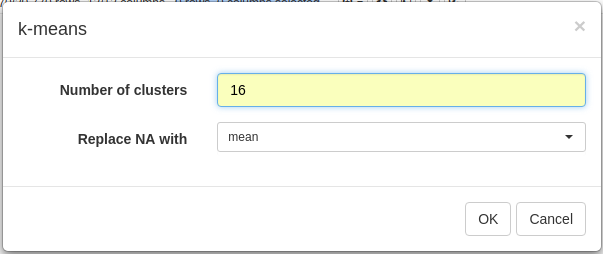
\includegraphics[scale=0.4]{kmeanstool.png}
   \label{kmeanstool}
\end{figure}

На клиенте в инструменте \texttt{KmeansTool}, который показан на рисунке~\ref{kmeanstool}, считываются следующие аргументы:
\begin{itemize}
\item количество кластеров, на которые нужно разбить данные;
\item функция замены \emph{NA} в данных.
\end{itemize}

Данные аргументы и ключ сессии актуального \texttt{ExpressionSet} отправляются на сервер в соответствующую функцию \texttt{kmeans}, код которой можно увидеть на листинге~\ref{kmeans}. Также как и в \texttt{pcaPlot}, здесь сначала заменяются \texttt{NA} на соответствующие данной функции значения, так как в этом случае \texttt{NA}-значения мешают вычислить среднее среди векторов. После данные отправляются в стандартную функцию \texttt{kmeans} пакета \emph{stats}~\cite{stats}. Результат возвращается как список соответствия каждого гена определенному кластеру, который приходит на клиент в \emph{JSON}-формате и отрисовывается как новая цветовая аннотация к строкам. Пример такой аннотации можно увидеть на рисунке~\ref{kmeansexample}.

\begin{lstlisting}[float=!h,caption={Кластеризация методом kmeans},label={kmeans},language=R]
kmeans <- function(es, columns = c(), rows = c(), k, replacena = "mean") {
  assertthat::assert_that(k > 0)

  rows <- getIndicesVector(rows, nrow(exprs(es)))
  columns <- getIndicesVector(columns, ncol(exprs(es)))
  data <- replacenas(data.frame(exprs(es))[rows, columns], replacena)

  data <- t(scale(t(data)))
  while (sum(is.na(data)) > 0) {
    data <- replacenas()
    data <- t(scale(t(data)))
  }

  km <- stats::kmeans(data, k)
  res <- data.frame(row.names = row.names(exprs(es)))
  res[["cluster"]] <- NA
  res[names(km$cluster), "cluster"] <- as.vector(km$cluster)
  return(toJSON(as.vector(km$cluster)))
}
\end{lstlisting}

\begin{figure}[h]
  \caption{Результат работы инструмена \texttt{KmeansTool} на данных GSE14308}
  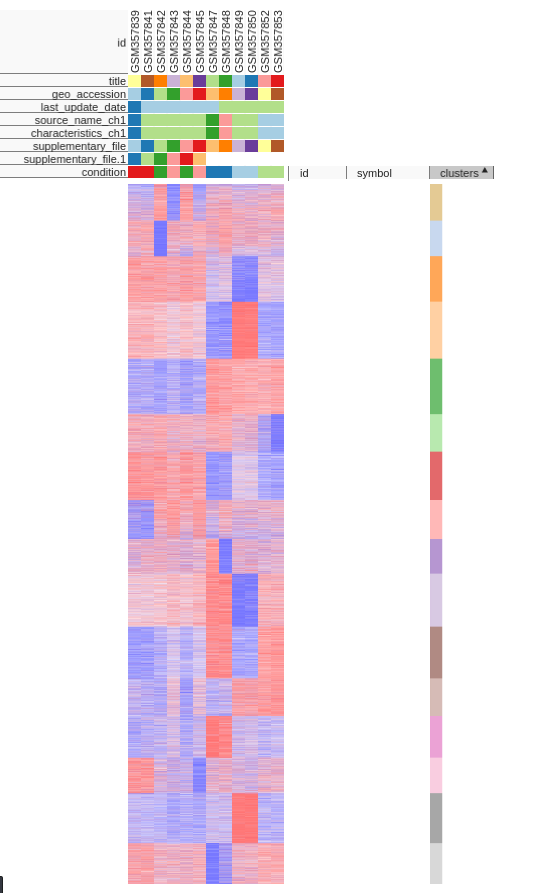
\includegraphics[scale=0.4]{kmeansexample.png}
  \label{kmeansexample}
\end{figure}

\subsection{Анализ дифференциальной экспрессии}
Инструмент предназначен для анализа дифференциальной экспрессии: экспрессия генов сравнивается в двух группах образцов, и вычисляются несколько статистических характеристик, показывающих, насколько случайны различия этих групп.

\begin{figure}[h]
  \caption{Графический интерфейс инструмента \texttt{LimmaTool}}
  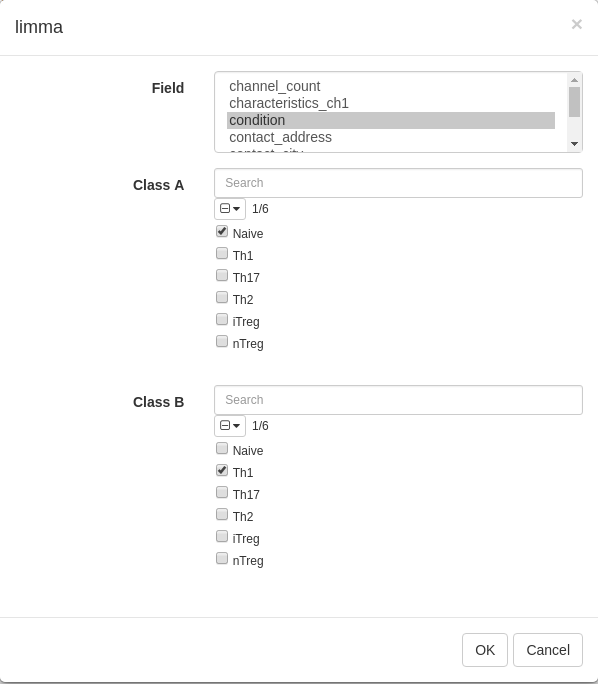
\includegraphics[scale=0.4]{limmatool.png}
  \label{limmatool}
\end{figure}

На клиенте, в инструменте, показанном на рисунке~\ref{limmatool}, осуществляется получение следующих аргументов:
\begin{itemize}
\item какие аннотации образцов участвуют в сравнении;
\item какая комбинация значений указанных выше аннотаций обозначает класс A;
\item аналогично для класса B.
\end{itemize}

Далее происходит подготовка аргументов к отправке на сервер: образцы разбиваются по выбранным аннотациям на три группы: A, B и не участвующие в сравнении.
Список соответствия образцов классам и ключ сессии, содержащей актуальный \texttt{ExpressionSet}, отправляются на сервер.

Аргументы приходят в функцию \texttt{limmaAnalysis}, код которой можно увидеть на листинге~\ref{limmaAnalysis}. Прежде чем использовать функцию \texttt{de} (\emph{differential expression}), реализованную в пакете \emph{limma}~\cite{limma}, которая помогает увидеть, насколько случайны различия между образцами, гены которых находятся в разных условиях, необходимо дополнить аннотацию образцов списком, содержащим идентификаторы классов сравнения.

Построенный дизайн сравнения передается в функцию \texttt{de}, которая возвращает матрицу статистических характеристик к каждому гену.
Эта матрица далее сериализуется в \emph{ProtoBuf} и записывается в файл.

\begin{figure}[h]
  \caption{Результат работы инструмента \texttt{LimmaTool} на данных GSE14308}
  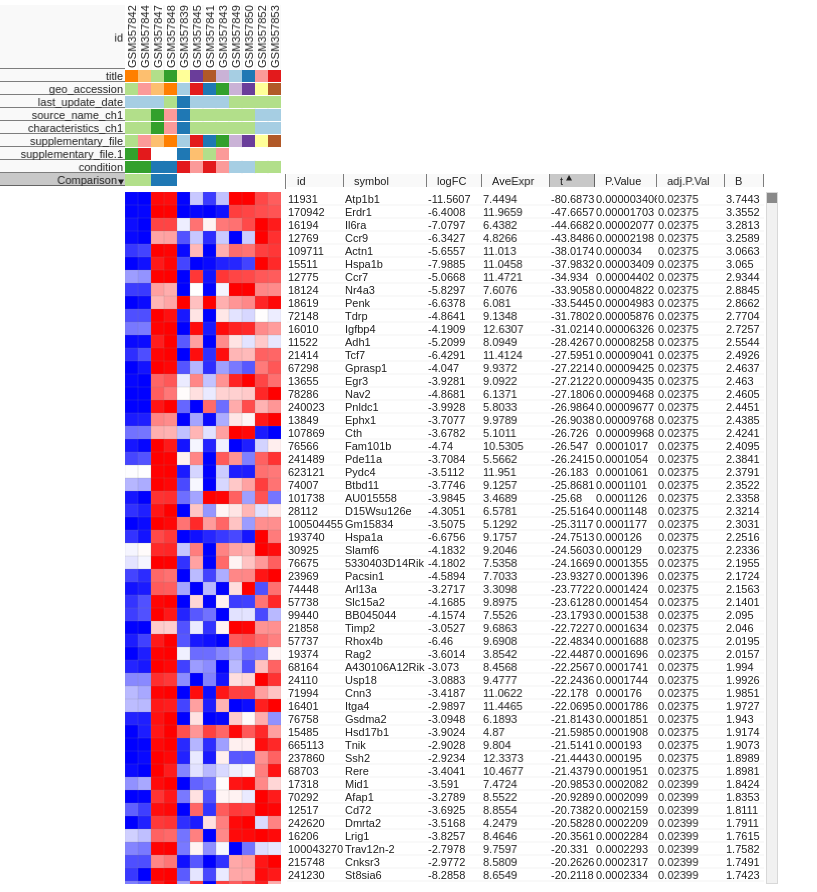
\includegraphics[scale=0.4]{limmaexample.png}
  \label{limmaexample}
\end{figure}

Клиент, получив ключ временной \emph{OpenCPU}-сессии, читает файл с сериализованной в \emph{ProtoBuf} матрицей результатов, которые с помощью \emph{protobuf.js} разбираются и после отрисовываются в виде аннотации к строкам. Результат работы можно увидеть на рисунке~\ref{limmaexample}.

\begin{lstlisting}[float=!h,caption={Реализация анализа дифференциальной экспрессии в R-пакете phantasus},label={limmaAnalysis},language=R]
limmaAnalysis <- function(es, rows = c(), columns = c(), fieldValues) {
  assertthat::assert_that(length(columns) == length(fieldValues) || length(columns) == 0)
  rows <- getIndicesVector(rows, nrow(exprs(es)))
  columns <- getIndicesVector(columns, ncol(exprs(es)))
  fieldName <- "Comparison"
  fieldValues <- replace(fieldValues, fieldValues == '', NA)
  new.pdata <- pData(es)[columns,]
  new.pdata[[fieldName]] <- as.factor(fieldValues)
  new.pdata <- new.pdata[!is.na(new.pdata[[fieldName]]),]
  new.sampleNames <- row.names(new.pdata)
  es.copy <- es[rows, new.sampleNames]
  pData(es.copy) <- new.pdata
  fData(es.copy) <- data.frame(row.names=rownames(es.copy))
  es.design <- model.matrix(~0 + Comparison, data = pData(es.copy))
  colnames(es.design) <- gsub(pattern = fieldName,
                              replacement = '',
                              x = make.names(colnames(es.design)))
  fit <- lmFit(es.copy, es.design)
  fit2 <- contrasts.fit(fit, makeContrasts(B - A,
                                           levels=es.design))
  fit2 <- eBayes(fit2)
  de <- topTable(fit2, adjust.method="BH", number=Inf)
  de <- de[row.names(fData(es.copy)),]
  f <- tempfile(pattern = "de", tmpdir = getwd(), fileext = ".bin")
  writeBin(protolite::serialize_pb(as.list(de)), f)
  f
}
\end{lstlisting}

\section{Инфраструктура проекта phantasus}
\subsection{Структура git-репозитория}
Как следует из главы об архитектуре проекта, проект состоит из двух составляющих:
\begin{itemize}
\item \emph{phantasus.js} --- \emph{fork} репозитория \emph{morpheus.js}~\cite{morpheus};
\item \emph{phantasus} --- репозиторий для \emph{R}-пакета.
\end{itemize}
Внутри репозитория \emph{phantasus} находится подмодуль для репозитория \emph{phantasus.js}.
Соответственно, чтобы загрузить целиком весь проект достаточно вызвать команду из листинга~\ref{clonerepo}.
\begin{lstlisting}[float=!h,language=bash,label={clonerepo},caption={Клонирование репозитория проекта phantasus}]
  git clone --recursive https://github.com/ctlab/phantasus.git
\end{lstlisting}

\subsection{Запуск приложения}
На данный момент существует два варианта запуска приложения \emph{phantasus}. В данном разделе будут описаны оба.
\subsubsection{Единый R-пакет phantasus}
Так как проект теперь существует в виде  единого \emph{git}-репозитория, его легко можно использовать как полноценный R-пакет, содержащий в себе в том числе и файлы для веб-приложения.
С помощью функции, представленной на листинге~\ref{serve.R}, можно запускать веб-приложение phantasus непосредственно из R.
\lstinputlisting[float=!h,language=R,label={serve.R},caption={Функция для запуска приложения из R}]{listings/serve.R}

Соответственно, чтобы запустить приложение, необходимо выполнить код, представленный на листинге~\ref{launchR} и перейти на \texttt{http://localhost:8000} в браузере.

\begin{lstlisting}[float=!h,language=R,label={launchR},caption={Запуск приложения в качестве R-пакета}]
library(phantasus)
example(servePhantasus)
\end{lstlisting}

\subsubsection{Docker-образ phantasus}
На \texttt{hub.docker.com} существует автоматический репозиторий, привязанный к \emph{git}-репозиторию \emph{phantasus}. Для каждой перекомпиляции он использует Dockerfile с листинга~\ref{dockerfile}, расположенный в репозитории.

На данный момент существуют две ветки Docker-образа:
\begin{itemize}
\item \emph{master} --- компиляция происходит из \emph{master}-веток составляющих проекта, чаще всего эти скомпилированные образы стабильны и отправляются в открытый доступ для использования;
\item \emph{develop} --- компиляция происходит из \emph{develop}-веток составляющих проекта, эти образы используются для тестирования всего приложения в целом, тестирования нового функционала и не предназначены для использования на серверах.
\end{itemize}

Чтобы загрузить \emph{Docker}-образ, нужно воспользоваться командой с листинга~\ref{dockerpull}
\begin{lstlisting}[float=!h,language=bash,label={dockerpull},caption={Загрузка Docker-образа phantasus}]
  docker pull dzenkova/phantasus
\end{lstlisting}

Для запуска \emph{Docker}-контейнера, необходимо воспользоваться командой с листинге~\ref{launchdocker}.
\begin{lstlisting}[float=!h,language=bash,label={launchdocker},caption={Запуск Docker-контейнера}]
  docker run -t -d -p 80:80 -p 8004:8004 dzenkova/phantasus
\end{lstlisting}

\subsection{Кэш для данных из GEO}
Независимо от способа запуска, данные, загруженные из GEO, кэшируются в определенной папке (сейчас это неизменяемое значение: \texttt{/var/cache/phantasus}), чтобы не было необходимости перескачивать их заново.

\section{Настройка с помощью Apache}
В обоих из представленных вариантах запуска, приложение запускается в формате \emph{single-user}, соответственно, настройка деятельности приложения в формате \emph{multi-user} осуществляется возможностями \emph{Apache}

\subsection{Переадресация OpenCPU-сервера}
Как было сказано в разделе~\ref{opencpuintro} обзора, \emph{OpenCPU}-сервер работает быстрее в однопользовательском режиме. Сервер запускаетстся на определенном порту (например, 8001), после для корректной работы приложения, происходит переадресация запросов с \texttt{/ocpu} на \texttt{//localhost:8001/ocpu} и наоборот.

\subsection{Балансировщик для multi-user соединения}
Из-за того, что используется однопользовательский \emph{OpenCPU}-сервер, несколько людей, использующих веб-приложение \emph{phantasus} одновременно, вынуждены ждать, пока закончится запрос для одного.

Чтобы избежать такой ситуации, запускается четыре одинаковых экземпляра \emph{OpenCPU}-сервера и с помощью \emph{Apache}-балансировщика можно получать доступ к \emph{R}-серверу параллельно.

\chapterconclusion
В данной главе были рассмотрены реализованные инструменты и методы анализа:\begin{itemize}
\item загрузка данных из \emph{Gene Expression Omnibus};
\item метод главных компонент и его визуализация;
\item кластеризация методом \emph{kmeans};
\item анализ дифференциальной экспрессии. \end{itemize}

Также были описаны технические подробности реализации веб-приложения: инструкции для запуска, варианты использования и детали настройки веб-приложения на сервере.

%% Макрос для заключения. Совместим со старым стилевиком.
\startconclusionpage
В ходе данной работы были получены следующие результаты:\begin{itemize}
\item разработан способ взаимодействия между \emph{JavaScript}-клиентом и \emph{R}-пакетом с помощью технологии \emph{OpenCPU};
\item реализованы инструменты: \emph{PcaPlot}, \emph{kmeans}, \emph{limma}, --- их графическое представление на \emph{JavaScript} и \emph{R}-реализация;
\item добавлена поддержка загрузки и визуализации данных из \emph{Gene Expression Omnibus} по идентификатору;
\item все компоненты соединены в веб-приложении \emph{phantasus}. \end{itemize}
Веб-приложение \emph{phantasus} было выпущено в открытый доступ и им можно пользоваться по адресу \texttt{https://artyomovlab.wustl.edu/phantasus}, либо же запускать самостоятельно в виде \emph{R}-пакета или \emph{Docker}-контейнера, как это было описано в главе~\ref{implementation}.
Проект \emph{phantasus} используется в:\begin{itemize}
\item лаборатории Максима Артемова в Washington University in St. Louis;
\item лаборатории Laurent Yvan-Charvet в Universit\'e Nice Sophia Antipolis.
\end{itemize}

Также проект был продемонстрирован на семинаре по системной биологии в Сиднее (10-13 апреля 2017) и в Санкт-Петербурге (14-19 мая 2017).

Полученное веб-приложение соответствует всем поставленным в разделе~\ref{require} требованиям. 
\printmainbibliography

%% После этой команды chapter будет генерировать приложения, нумерованные русскими буквами.
%% \startappendices из старого стилевика будет делать то же самое
\appendix
\chapter{Протокол сериализации в ProtoBuf}\label{proto}
R-пакет protolite использует стандартный протокол сериализации, представленный на листинге~\ref{proto}. Этот же протокол было решено использовать и при сериализации на клиенте для однообразия и для корректного разбора сообщений как на клиенте от сервера, так и на сервере от клиента.
\lstinputlisting[float=!h,caption={}]{listings/message.proto}
\chapter{Dockerfile}\label{dockerfile}
\lstinputlisting[float=!h,caption={Dockerfile для Docker-образа веб-приложения phantasus}]{listings/Dockerfile}

\chapter{Конфигурационный файл Apache}\label{apacheconf}
\lstinputlisting[float=!h,caption={}]{listings/phantasus.conf}
\end{document}
